\documentclass[12pt,oneside]{book}
\pagestyle{headings}

% Note that the line below could be modified to suit a
% particular system since the "geometry" package behaves
% differently in Unix, Windows and Mac, especially for the
% top margins.
% Adjust the parameter "top" (measuring the height of the
% space allocated to a header) and "headsep" (measuring
% the distance from the bottom of the header to the
% first line of text.
\usepackage[top=1.3in,left=1.5in,bottom=1in,right=1in,headsep=0.5in]{geometry}

\usepackage{setspace}
\onehalfspacing
%\doublespacing

% Headers and footers for thesis
\usepackage{fancyhdr}

\markboth{}{}
\newcommand\startchapter[1]{\chapter{#1}\thispagestyle{myheadings}}
\newcommand\startappendix[1]{\chapter{#1}\thispagestyle{myheadings}}
\newcommand\startfirstchapter[1]{\chapter{#1}}

% Manual addition of section to Table of Contents
\newcommand\TOCadd[1]{\newpage\phantomsection\addcontentsline{toc}{chapter}{#1}}

% Float Customization
\renewcommand{\floatpagefraction}{0.01}

% Customization of Tables of Contents and List of Figures/Tables
\usepackage{tocloft}
\renewcommand\cfttabpresnum{Table\ }
\renewcommand\cfttabnumwidth{0.75in}
\renewcommand\cftfigpresnum{Figure\ }
\renewcommand\cftfignumwidth{0.80in}
\newcommand{\HRule}{\rule{\linewidth}{0.5mm}}

% Long Table and decimal aligned columns
\usepackage{dcolumn}
\usepackage{longtable}
\usepackage{algorithm}
\usepackage[noend]{algpseudocode}
\usepackage{amsfonts}
\usepackage{ragged2e}
\usepackage{tabularx}
\usepackage{multirow}

% Mathematics support
\usepackage{amsmath,algorithm,algpseudocode}
\usepackage{amsthm}
\usepackage{amssymb}
\usepackage{amsfonts,bm}

% Text Control
\usepackage{xspace}
\usepackage{textcase}

% Graphics
\usepackage{wasysym}
\usepackage{graphics}
\usepackage{graphicx}   % A package to allow insertion of
                        % external image files
                     


\usepackage{algorithm}
\usepackage{algpseudocode}
\usepackage{amsfonts}

\begin{document}

% Front Matter
\input frontmatter/fm

\newpage

	\startfirstchapter{Introduction}
\label{chapter:introduction}

The development of a personalized learning system began with the creation of an intelligent tutoring system (ITS) \cite{brusilovsky2003adaptive,koedinger1997intelligent,vanlehn2005andes,woolf2010building}. However, ITSs are primarily rules-based which need domain experts to manually specify every possibility that a system might face so it could present appropriate learning actions. This presented a massive combinatorial, labor-intensive challenge as every possible learning path would have to be explicitly specified \cite{lan2016contextual}.\par 

In recent years, machine learning has shown that it has the potential to personalize learning and scale for several courses and students. Machine learning based systems use data to personalize learning actions for each student without the need to explicitly specify learning actions for each individual student. Example of actions could be reading a chapter from a book or article, listening to a podcast, watching a video, or interacting with the system by answering quizzes. These systems are continuously learning from the data generated through students interactions with the system. Thus it has the potential to eliminate the challenges one would face with a traditional ITS  \cite{lan2016contextual}. \par 

\textbf{The goal of this project is to design a learning algorithm, which could adapt based on student's feedback to help them learn effectively}. \par 

\section{Use Case \label{chap1:useCase}}

There is no universal best way to explain a topic. The best way is subjective to every student. Unless we explore different ways to teach a topic, we cannot find a policy which would help map different students to explanations conducive for them. Once, we have such a policy we can use it to teach every student effectively. \textbf{This is the exploration-exploitation dilemma where there is a trade-off between exploration (exploring non-stationarity in a student's preferences) and exploitation (maximize a student's satisfaction over a period of time)} \cite{agarwal2009online}. For example, an adaptive teaching system should present different explanations knowing a student's preference for learning. However, unless we try different ways of teaching it is not possible to say with certainty whether or not an explanation would help a student learn effectively. We use the term adaptive teaching to avoid confusing it with adaptive learning used in machine learning literature. In the education domain, these terms are used interchangeably. \par 

We represent this use case as a contextual bandit problem. We use contextual information about the student such as their preferences to learn through \textit{visual, text, demo-based, practical, activity-based, step-by-step, lecture, audio-based explanations as well as self-evaluation and pre-assessment of students}. We also use contextual information about the content's used to teach a topic, by rating them in terms of \textit{ease of understanding, simplicity, intuitiveness, depth in teaching, conciseness, thoroughness, ratings, abstractness, hands-on, experimental}. A \textbf{content item or arms are different actions or ways a topic can be taught}. The reward would be the student's feedback to confirm their understanding of the topic they are trying to learn. The feedback can be through quizzes, interactions with a content item, tasks to name a few. \textbf{By pulling an arm, we obtain a reward drawn from some unknown distribution determined by the selected content item and the context. Our goal is to maximize the total cumulative reward}.  \par 

Let us make this more concrete by mapping this use case to teaching a class. In any school, a course comprises of multiple topics. However now instead of a single way to teach everyone, there would be multiple ways to teach. These different ways to teach are called content items. Student's give their feedback on the presented content. Behind the scenes, our learning algorithm takes information about the student \textit{(also referred to as student context)}, topic, content items\textit{(also referred to as content context)} to find the best way to teach a student. This project extends the most cited contextual bandit learning algorithm, LinUCB (Linear Upper Confidence Bound) \cite{li2010contextual} to enhance it for our use case. \par

\section{Motivation \label{chap1:motivation}}

The main problem with traditional education, which has been perpetual, is the enormous challenge teachers face for being responsible to ensure every student is able to acquire expertize in their subject even though students may come from diverse backgrounds and interest \cite{educauseReview}. In such classrooms learning has largely remained a one-size-fits-all experience in which the teacher selects a learning resource for all students in their class regardless of their diversity in needs, understanding, ability, preferred learning style, and prior knowledge. It is not feasible for teachers to ensure their explanations can cater to all students. Hence there is a need for a system which could personalize teaching for students to help them learn effectively as well as increase course engagement and progression.\par

Such systems would be adaptive, recognize different levels of prior knowledge among students, as well as course progression based on a student's skill and feedback from learning. This could change teachers responsibility from a provider to a remediator and facilitator in teaching. These would adapt to individual student's learning patterns instead of a student having to adjust to the way of teaching. They would provide timely and comprehensive data-driven feedback to recognize potential challenges that students might come across as the course progresses.\par

\section{Contribution}

We present a novel baseline algorithm for our proposed adaptive teaching methodology which learns from students and contents for each topic to create a personalized learning path for every student. It adapts dynamically based on student's feedback and learning preferences.  \par

We also provide a skip feature which is meant to keep a student engaged to increase their retention as well as provide feedback to teachers by recognizing the challenges faced by a student early in the course. Our online learning algorithm gives close to optimal results over a synthesized unbiased heterogeneous dataset. \par

\newpage
\section{Organization}

% \begin{description}
Chapter 1 provided a brief overview of our use case along with the need for an adaptive teaching system and how this project contributes to realizing it. Chapter 2 introduces the technical concepts used to represent our use case along with the algorithm we customize for adaptive teaching. Chapter 3 describes prior work related to our use case using different approaches and how our work compares to them. Chapter 4 explains the algorithm created for adaptive teaching along with the skip feature. Chapter 5 describes the experimental setup along with the dataset synthesized to evaluate our algorithm. It also explains the evaluation strategy followed to examine our results. Chapter 6 presents the results of our experiments and compares our learning algorithm with respect to the best possible policy. Chapter 7 concludes this project by summarizing the contributions and outlines possible avenues for future work.
% \end{description}
    \startchapter{Preliminaries}
\label{Preliminaries}

This chapter briefly explains the key concepts used in this project.

\section{Multi-armed bandit \label{chap2:bandits}}

Multi-armed bandit is a problem setting where an agent makes a sequence of decisions in time $1, 2, ..., T$. At each time $t$ the agent is given a set of $K$ arms to choose and has to pull an arm. As a feedback for pulling an arm, it receives a reward for that arm, while the rewards of other arms cannot be determined. Problems represented as multi-armed bandits are stateless. They can be stochastic or adversarial. In a stochastic environment the reward of an arm is sampled from some unknown distribution, and in an adversarial setting the reward of an arm is picked by an adversary and is may be sampled from a distribution \cite{zhou2015survey}. In this project, we assume the problem setting as stochastic. \par

Personalized recommender systems recommend items (e.g., movies, news articles, web advertisements) to their users based on their predicted preference for these items. The feedback received from users response helps the system improve their prediction \cite{adomavicius2005toward}. However, to improve the quality of recommendations an item has to first be recommended. If an item is never recommended to users, the system cannot evaluate the feedback to improve it's quality of predictions on these items. Such problems where there is some information about the users which can be used to improve the quality of predictions without can be represented as a contextual bandit problem  \cite{vermorel2005multi}.

\section{Contextual Bandit \label{chap2:cb}}

In the theory of sequential decision-making, contextual bandit problems \cite{tewari2017ads} are placed between multi-armed bandit problems \cite{bubeck2012regret} and full-blown reinforcement learning (usually modeled using Markov decision processes with discounted or average reward to take optimal actions) \cite{sutton1998introduction}. Traditional bandit algorithms do not use any side-information or context. However, contextual bandit algorithms use context to learn and map contexts to appropriate actions. Since bandit algorithms only have a single state they do not have to consider the impact of their actions future states. Nevertheless, in many practical domains, such a problem setting is useful. This is true when the learner's action have limited impact on future contexts. In such a problem setting contextual bandit algorithms have shown great promise. Examples include web advertising \cite{abe1999learning} and personalized news article recommendation on web portals  \cite{li2010contextual,greenewald2017action}. \par

Formally a contextual bandit problem is a repeated interaction which takes place over $T$ rounds. At each round $t = 1,2,...T$ the environment reveals contexts $x_t \in X$ about the user and the available actions which are used by the learner to pick an action $a_t \in A$ which gives a reward $r_t$ revealed by the environment. The goal of the learner is to choose an action which would maximize cumulative reward $\sum_{t=1}^{T} r_t$. \par

We will now translate this problem setting for our adaptive teaching use case in which an algorithm $A$ which proceeds in discrete rounds $t = 1,2,3,...$. In round t: 
\begin{enumerate}
\item The algorithm observes the student context $x_s$ and a set $A_t$ of content items together with their feature vectors $x_{c}$ for $a \in A_t$. $X_{t}$ encapsulates $x_s$ and the context ${x_c}$ of all content items available in round $t$.
\item Based on observed rewards in previous rounds, $A$ chooses an arm $a_t \in A_t$. The arm $a_t$ is estimated to have the highest expected reward. In a stochastic setting, the expected reward is given as the inner product of an unknown arm-dependent parameter $\theta_{a,t}$ and the context $x_{t,a}$, that is, $E[r_{t,a}|\mathbf{x_{t,a}}] = x^{T}_{t,a}\mathbf{\theta_{t,a}}$. 
\item The student reveals the received reward $r_t$ for arm $a_t$ whose expectation depends on both the context $X_t$ and the arm $a_t$. 
\item The algorithm then improves it's content item selection strategy with the new observation $(x_t,a_t,r_t)$. It is important to emphasize here that no feedback namely, reward $r_{t}$ is observed for unchosen arms $a \neq a_t$ \cite{li2010contextual}.
\end{enumerate}

\section{Upper Confidence Bound (UCB) \label{chap2:UCB}}

An unavoidable challenge in bandit algorithms is to find the right balance between exploration and exploitation (Section \ref{chap1:useCase}). Upper Confidence Bound (UCB) comprises of a family of algorithms which try to find the best trade-off between exploration and exploitation. It is based on the principle of \textit{being optimistic} by choosing actions which have the highest potential for reward. The intuitive reason that this works is that when acting optimistically, one of two things happens. Either the optimism was well justified, in which case the learner is already acting optimally, or the optimism was not justified. In the latter case, the algorithm takes some action that they believed might give a reward when in fact it does not. If this happens sufficiently often, then the algorithm will learn the true reward of this action and not choose it in the future \cite{banditalgs}. UCB algorithms estimate the expected reward for each arm by adding estimated sample mean of an arm with it's upper confidence bound. \par

We will refer to Figure \ref{UCB} as an example to understand UCB. Let us assume we have three arms $a_1, a_2, a_3$. The reward distribution for each arm after several rounds is a Gaussian distribution $Q$ with mean $\mu$ and standard deviation $\sigma$. The y-axis is the probability of obtaining a certain reward for these arms. \par

\begin{figure}[h]
    \centering
    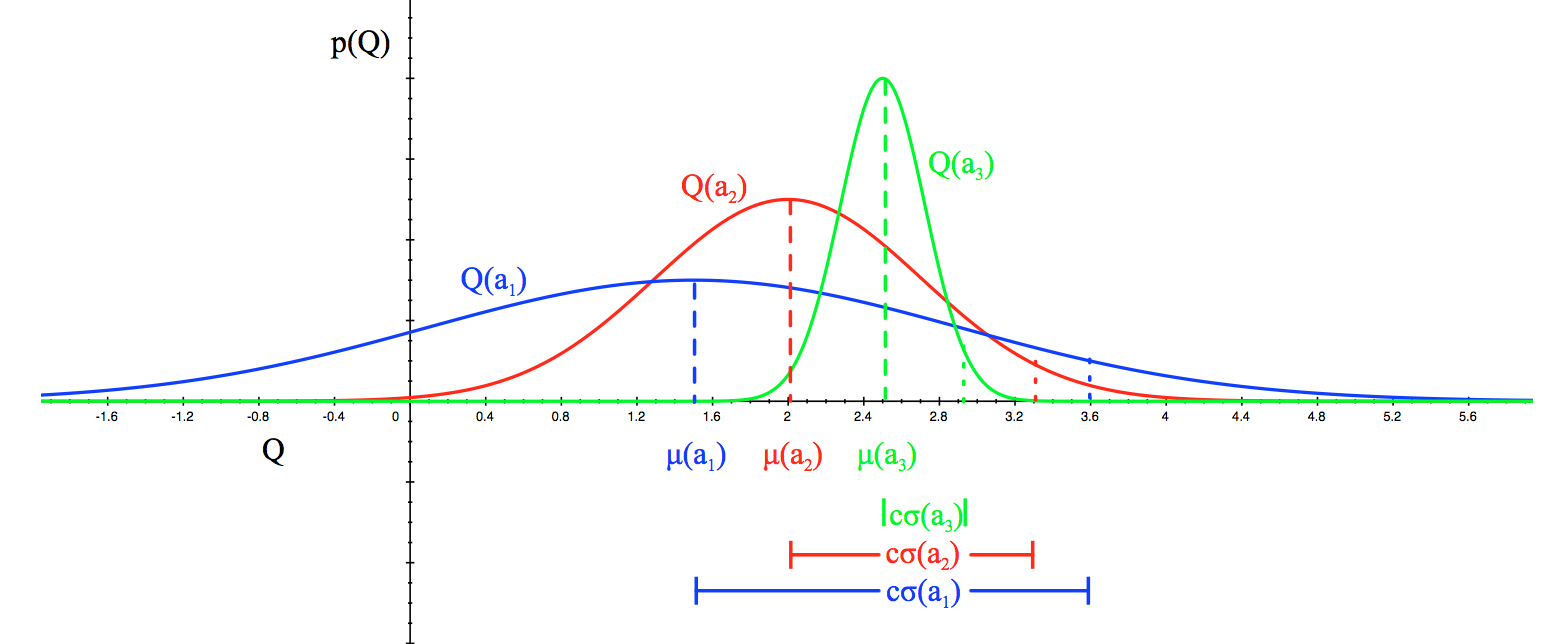
\includegraphics[scale=0.28]{Figures/UCB.png}
    \caption{An example: UCB}
    \cite{dsilver}
    \label{UCB}
\end{figure}

The upper confidence bound for each arm is given by $c\sigma(a_i)$. The distribution shows that the sum of the expected mean and upper confidence bound is highest for $a_1$. Hence the UCB algorithm will select $a_1$.
The reward received will reduce uncertainty around $a_1$. So for the next round, the algorithm once again finds the arm with the highest sum for the expected mean and upper confidence bound. This is repeated for $T$ rounds \cite{ankitmab}.

\section{Linear Upper Confidence Bound (LinUCB) \label{chap2:linUCB}}

LinUCB is a way to apply UCB to a more general contextual bandit setting where the UCB of each arm is computed efficiently by assuming the reward is linear, given as $E[r_{t,a}|\mathbf{x_{t,a}}] = x^{T}_{t,a}\mathbf{\theta_{t,a}}$. The estimated expected mean is parameterized over the context $x_{a}$ for each arm $a$. At round $t$ this is given as $\widehat{\theta}^{T}_{a}x_{t,a}$. The upper confidence bound around each arm $a$ at round $t$ is given as $\sqrt{x^{T}_{t,a}A^{-1}_{a}x_{t,a}}$. Here, $A_a$ is the co-variance over the context data $x_{t,a}$ for each arm $a$ at round $t$.  \par

LinUCB introduces a hyper-parameter $\alpha$, which allows us to control exploration over arms. This is achieved by scaling the upper confidence bound by $\alpha$. A higher value of $\alpha$ encourages exploration. As a result, the algorithm would need more rounds to explore before it begins exploiting. We can now compute \textbf{the expected estimated reward for an arm $a$ at round $t$ as $p_{t,a} = \widehat{\theta}^{T}_{a}x_{t,a} + {\alpha} \sqrt{x^{T}_{t,a}A^{-1}_{a}x_{t,a}}$}  \cite{li2010contextual}.\par
    \startchapter{Related Work}
\label{chapter:problem}

Our use case could also be represented using a partially observed Markov decision process (POMDP) framework. POMDPs model the student's latent knowledge states and their transitions to learn a policy that will present an action that could maximize reward received over the long run (long-term learning outcome). Previous work applying POMDPs to personalized learning has had limited success. However, to create a personalized learning schedule using a POMDP can get complicated and intractable as the number of dimensions representing the states and actions grows. As a consequence of this curse of dimensionality, POMDPs have had a limited impact to personalize learning in large-scale applications which has a large number of students and learning actions \cite{lan2016contextual}. \par 

A more practical and tractable approach to personalized learning is to learn a policy, which maps contexts to actions using the multi-armed bandit (MAB) framework, which is more suitable for our use case. This makes it more practical than the POMDP framework in large-scale educational applications \cite{lan2016contextual}. \par

The work in \cite{liu2014trading} applies a MAB algorithm to educational games to find a trade-off between exploring learning resources to accurately estimate arm means, while also trying to maximize users test performance. Their approach is context-free and does not consider diversity among individual users. The work in \cite{mandel2014offline} collects data to find how students interact with the system to extract features as they play an educational game. It uses this knowledge to find a good teaching policy \cite{lan2016contextual}. \par 

The work in \cite{lan2016contextual} is focused on adaptive testing to assess students performance. They use contextual MAB to find questions to assess a student. The question depends on a student's response to earlier questions. At each round, they have all questions to assess a student. Contrary to that we only have a restricted set of content items available at each round. Our use case is focused on adaptive teaching to enable students to learn. \par

The works in \cite{clement2013multi,koedinger2013new} both uses expert knowledge to learn a teaching policy. The approach of \cite{clement2013multi}, in particular, uses domain expertize to reduce the set of possible actions a student can take. Our approach, in contrast, requires no expert knowledge and is fully data-driven \cite{lan2016contextual}. \par

Other works typically create a model for each component, namely student, knowledge, domain and use knowledge tracing \cite{corbett1994knowledge}, item response theory and zone of proximal development \cite{lord2012applications,reckase2009multidimensional,bergner2012model} to make better decisions. These different methods have similar predictive performance. However, they could have very different teaching policies. \cite{lan2016contextual}. While these results are different approaches to make the best prediction, none of them use machine learning to develop a policy learning algorithm.\par

\newlength{\savedunitlength}
\setlength{\unitlength}{2em}

\setlength{\unitlength}{\savedunitlength}
	\startchapter{Algorithm}
\label{chapter:algorithm}

This chapter presents the algorithm created for the adaptive teaching system. We first present the basic version of the algorithm (Section \ref{chap4:basic}). We then explain the skip feature (Section \ref{chap4:skip}), which could streamline learning. \par

The algorithm used is an extension of upper confidence bound (UCB)-based algorithms \cite{auer2002finite} (Section \ref{chap2:UCB}). These algorithms maintain estimates of the expected reward of each arm together with confidence bound around it. It then pulls the arm with the highest estimated reward which is equal to the sample mean plus the confidence bound. Based on the actual reward it updates the arms parameters iteratively after each pull to make a better decision in upcoming rounds. In this project we are using the most cited contextual bandit algorithm, namely LinUCB (Section \ref{chap2:linUCB}).  \par

Before we dive in it is important to note, that to better understand the algorithm we have divided the explanation into two halves. \textit{The first half explains the overall flow without skipping whereas the second explains in-depth the function calls made in the first half along with skipping}. We are using bandit terminology to explain. \textbf{Arm} refers to a content item. \textbf{Payoff} is the algorithms upwardly biased estimate of the expected reward, where the bias is due to the algorithms use of an upper confidence bound rather than using the sample mean directly. A \textbf{round} comprises of computing the expected payoff for each content item; then presenting a content item with maximum expected payoff and getting student feedback for the content item. \par

Below are the notations used in the algorithm.

\begin{table}[H]
\centering
\label{Table 1 : Notations}
\begin{tabularx}{\linewidth}{ @{} r X @{} }
     \hline
     Symbol & Meaning \\
     \hline
     $\alpha$  & Parameter to scale Confidence bound.  \\ 
     $C$ & Confidence threshold to skip. \\
     $\mathbf{x_s}$ & Student context vector. \\
     ${x_c}$ & Content items context matrix for a topic. \\
     $\mathbf{x_t}$ & Context vector at round $t$. \\
     $X_{t}$ / $X^{i}_{t}$  & Context at round $t$. It combines $\mathbf{x_s}$ and all available $x_c$ for topic $i$. \\
     $X^{i+1}_{t}$  & Context at round $t$. It combines $\mathbf{x_s}$ and all available $x^{i+1}_c$ for topic $i+1$. \\
     $x^{i+1}_c$ & Content items contexts for topic $i+1$. \\
     $a$ & An arm $a$ for topic $i$.\\
     $a'$ & An arm $a'$ for topic $i+1$.\\
     $A_t$ & Arms available at round $t$. \\
     $A^{i+1}_{t'}$ & Arms available for topic $i+1$ at round $t'$. \\
     $a^{i+1}_t$ & Arm $a$ for topic $i+1$ at round $t$. \\
     $t$ & Current round $t$. \\
     $t'$ & Possible next round $t'$. \\
     $i$ & Topic being taught. \\
     $i+1$ & Next Topic in the sequence. \\
     $p_{t,a}$ & Expected payoff from arm $a$  at round $t$. \\ 
     $p^{i}_{t,a}$ & Expected payoff from arm $a$ at round $t$ for topic $i$. \\
     $p^{i+1}_{t',a'}$ & Expected payoff from arm $a'$ at round $t'$ for next topic $i+1$. \\
     $X$ & Input features for skip classifier. \\
     $Y$ & Label to train the skip classifier. \\ 
   \hline   
\end{tabularx}
\caption{Algorithmic notations}
\end{table}

\textbf{Note}
\begin{itemize}
    \item We are always on the current topic $i$, unless we explicitly specify next topic $i+1$.
    \item All vectors are \textbf{bold} faced lower cased.
    \item All sets are plain faced.
\end{itemize}

\begin{algorithm}
\caption{Teach with LinUCB}
\begin{algorithmic}[1]
 \State \textbf{Hyper Parameters :} $\alpha$ $\in$  $\mathbb{R_+}$
    \State \qquad \qquad \qquad \qquad \qquad \, $C$ : Confidence threshold to skip 
    \State \textbf{Inputs :} Student context $\mathbf{x_s}$ and content context $x_c$ of available arm $a \; \in A_t$ for topic $i$ at round $t$
    \State Prepare context $X_{t} = \;\begin{pmatrix} \mathbf{x_s} \\ x_c \end{pmatrix}$
    \State skip-enabled $\gets$ False
    \While {$A_t \neq \emptyset$}
    \State $a^{i}_{t}$ , $p^{i}_{t,a} \gets$ \; \Call{Expected-Payoff}{$X_{t}$,$A_t$}
    \State skip-decision , $p^{i+1}_{t',a'} \gets$ \Call{SkipTopic}{$\mathbf{x_s}$, $p^{i}_{t,a}$, $i$}
    \If{skip-decision and skip-enabled is True}
    \State Move to next topic $i \gets i+1$
    \State \textbf{break}
    \Else 
    \State Pull arm $a_t$ and observe reward $r_{t}$
    \State $A_{a_t} \gets A_{a_t} + \mathbf{x_{t,a_t}x^{T}_{t,a_t}}$
    \State \bm{$b_{a_t}$} $\gets$ \bm{$b_{a_t}$} + $r_{t}\mathbf{x_{t,a_{t}}}$
    \State label $\gets$ \Call{setlabel}{$r_t$}
    \State \Call{Train}{$\mathbf{x_s}$, $p^{i}_{t,a}$, $p^{i+1}_{t',a'}$,label}
    \State $t \gets t+1$
    \EndIf 
    \If{$r_t \neq 1$}
    \State Remove $a_t \; \in A_t$
    
    \State skip-enabled $\gets$ True
    \Else 
    \State Move to next topic : $i \gets i+1$
    \State \textbf{break}
    \EndIf 
    \EndWhile
    \algstore{myalg}
\end{algorithmic}
\end{algorithm}

\section{Basic Version \label{chap4:basic}}

The basic version is without skipping. It explains the main flow of the algorithm. The next section explains the functions used along with skipping. \par

The algorithm requires two hyper-parameters to be configured. The first one is $\alpha$ which scales the confidence bound (Section \ref{chap2:linUCB}). The second hyper-parameter is the confidence threshold $C$ which decides confidence threshold that must be exceeded to skip a topic. Skipping is a feature to help students who are unlikely to learn from content items available for a topic. It is meant to streamline learning. This could also be used by teachers to recognize topics that should be addressed in class. \par

We now explain how LinUCB (Section \ref{chap2:linUCB}) helps the algorithm decide an arm to pull. Before we recommend a content item to a student, we need to prepare context $X_t$ for the round $t$. It is prepared by combining the student context $\mathbf{x_s}$ with content items context $x_c$ for the topic $i$ being taught. With the context $X_t$ and arms $A_t$, we use LinUCB to compute the expected payoff from each arm and return the arm $a^{i}_t$ with the maximum expected payoff $p^{i}_{t,a}$ which must be pulled for topic $i$ at round $t$. \par 

Assuming the classifier does not recommend skipping, a student is presented with the content item $a_t$ for topic $i$. After being taught the student sends a reward $r_t$ to complete the round $t$. Now the round $t$ is complete we update the arm parameters $A_{a_t}$ , $\mathbf{b_{a_t}}$ of the arm pulled. We then use this reward ${r_t}$ to train the skip classifier to make better predictions in upcoming rounds. The features for the classifier comprise of a student's contextual information $\mathbf{x_s}$, expected payoff $p^{i}_{t,a}$ from the current topic $i$ and the expected payoff $p^{i+1}_{t',a'}$ for the topic $i+1$. \par

If no reward $r_t$ was sent by the student $\mathbf{x_s}$, then it implies the student was unable to understand topic $i$. In which case the algorithm removes the presented arm $a_t$ and remains on the same topic $i$. However if a reward $r_t$ was sent, then the student is moved to the next topic $i+1$. This completes the first half. The second half explains the functions briefly described above. \par

\section{With Skipping \label{chap4:skip}}

\begin{algorithm}                     
\begin{algorithmic} [1]                   % enter the algorithmic environment
\algrestore{myalg}
    \Function{SkipTopic}{$x_s$, $p^{i}_{t,a}$, $i$}
        \State Get next topic $i+1$ from topic $i$
        \State Get arms $A^{i+1}_{t'}$ and content context $x^{i+1}_{c}$ for topic $i+1$ 
        \State Prepare context vector $X^{i+1}_{t'} =\; \begin{pmatrix} x_s \\ x^{i+1}_{c} \end{pmatrix}$
        \State $a^{i+1}_{t'}$ , $p^{i+1}_{t',a'} \gets$ \Call {expected-payoff}{$X^{i+1}_{t'}$,$A^{i+1}_{t'}$}
        \State skip-decision $\gets$ \Call{predict}{$x_s$, $p^{i}_{t,a}$, $p^{i+1}_{t',a'}$} to decide on skip
        \State \Return skip-decision , $p^{i+1}_{t',a'}$
    \EndFunction
    
    \Function{expected-payoff}{$X_t$,$A_t$}
        \For {$a\; \in\; A_t\;$} 
        \State Get $x_{t,a}\; \in \; X_t$
            \If {$a$ is new}
                \State $A_a \gets I_d$ (d-dimensional identify matrix)
                \State \bm{$b_a$} $\gets 0_{d \times 1}$ (d-dimensional zero vector)
            \EndIf
            \State $\widehat{\theta}_a \gets A^{-1}_{a}b_a $
            \State $p_{t,a} \gets \widehat{\theta}^{T}_{a}x_{t,a} + \alpha \sqrt{x^{T}_{t,a}A^{-1}_{a}x_{t,a}}$
        \EndFor
        \State Choose arm $a_{t}$ = arg max$_{a \in A_t} p_{t,a}$ with ties broken arbitrarily
        \State \Return $a_t , arg max p_{t,a}, $
    \EndFunction
    
    \Function{predict}{$x_s$, $p^{i}_{t,a}$, $p^{i+1}_{t',a'}$}
        \State X $\gets {x_s} \; , ${i+1}$ \; , p^{i}_{t,a} \; , p^{i+1}_{t',a'}$
        \State Y , confidence-score $\gets$ Prediction \; from \; classifier
        \If{confidence-score \textless C}
        \State decision $\gets$ 0
        \EndIf
        \State \Return \; decision , confidence-score
    \EndFunction
    
    \Function{train}{$x_s$, $p^{i}_{t,a}$, $p^{i+1}_{t',a'}$, label}
        \State $X \gets x_s , p^{i}_{t,a} , p^{i+1}_{t',a'} $ , topic ,
        \State $Y \gets$ label
        \State Train online SGD classifier
    \EndFunction
    
    \Function{setLabel}{$r_t$}
        \If{$r_t$ is 0}
        \State $label \gets 1$
        \Else
        \State $label \gets 0$
        \EndIf
        \State \Return label
    \EndFunction
    
\end{algorithmic}
\end{algorithm}

On line 6 (Section \ref{chap4:basic}) of the algorithm we get the expected payoff $p^{i}_{t,a}$ estimated on pulling the arm $a^{i}_t$ for the current topic $i$. Now to decide whether or not it should pull the arm or move to the next topic it calls the skip topic function. \par

The \textit{SKIPTOPIC} function takes the student context $\mathbf{x_s}$, the expected payoff $p^{i}_{t,a}$ for pulling arm $a$ at round $t$ for topic $i$ and the current topic $i$. It uses the topic $i$ to get a reference to the next topic $i+1$. Through the topic ${i+1}$ it gets content items $A^{i+1}_{t'}$ and context data $x^{i+1}_{c}$ associated those content items. After combining the contexts to prepare $X^{i+1}_{t'}$ 
it gets the maximum expected payoff $p^{i+1}_{t',a'}$ and the arm $a^{i+1}_{t'}$ to pull by passing the context vector $X^{i+1}_{t'}$ and arms available for next topic $A^{i+1}_{t'}$. The expected payoff function returns an arm with the maximum estimated payoff. Skip topic function then calls the skip classifier to predict a skip-decision for the student context $\mathbf{x_s}$, along with the expected payoff from the current and the next topic to make a prediction.

The \textit{EXPECTED-PAY0FF} function takes the context $X_t$, along with the arms $A_t$ available at round $t$. After an arm $a_t$ is initialized with parameters $A_a , b_a$ they are used to calculate the expected mean $\widehat{\theta}^{T}_{a}x_{t,a}$ and confidence bound $\sqrt{x^{T}_{t,a}A^{-1}_{a}x_{t,a}}$ for the arm. The confidence bound is scaled by $\alpha$. The expected mean and the scaled confidence bound are added to give the expected payoff $p_{t,a}$ for arm $a$ at round $t$. It then finds an arm $a$ with maximum expected payoff $p_{t,a}$ and returns the expected payoff along with the arm $a$ to be pulled. \par

The \textit{PREDICT} function is used to predict whether the student should be moved to the next topic $i+1$ or should remain on the same topic $i$. It combines student context vector $\mathbf{x_s}$, the expected payoff $p^{i}_{t,a}$ for the current topic $i$ and the expected payoff $p^{i+1}_{t',a'}$ for the next topic $i+1$ to prepare a feature vector $X$. It then gets a prediction from the binary supervised online support vector classifier with hinge loss to make a prediction $Y$ and a confidence-score for it's prediction. If the confidence-score is less than the confidence threshold, then set the $decision$ variable is set to 0 which implies no skipping. This is because a confidence score lower than the threshold implies that the classifier is not sufficiently confident about it's prediction. \par

The \textit{TRAIN} function is used to train the skip classifier to make better predictions. Similar to the predict function it combines student context vector $\mathbf{x_s}$, the expected payoff $p^{i}_{t,a}$ for the current topic $i$ and the expected payoff $p^{i+1}_{t',a'}$ for the next topic $i+1$ to prepare a feature vector $X$. It sets the $label$ to the output $Y$. Together they train the skip classifier. \par

The \textit{SETLABEL} function is used to set the $label$ to train the skip classifier. If the reward $r_t$ for round $t$ is set to 0 then the $label$ is set to 1. This implies that since staying on the same topic did not give any reward, it would have been better to skip. If the reward $r_t$ for round $t$ is set to 1, then the $label$ is set to 0. This implies that staying on the same topic was a good decision. The set $label$ is then returned. \par
	\startchapter{Experiments}
\label{chapter:Exp}

This chapter explains the dataset (Section \ref{chap5:dataset}) used to evaluate the learning algorithm. It then describes the environmental setup (Section \ref{chap5:environment}) used for these experiments. The next section explains how we evaluate our algorithm (Section \ref{chap5:evaluationStrategy}) in absence of pre-existing benchmarks using an omniscient policy (Section \ref{chap5:omniscientPolicy}). This is followed by sections which explain how the learning algorithm (Section \ref{chap5:learningAlgorithm}) and the skip feature (Section \ref{chap5:skipTopics}) work in these experiments.

\section{Dataset \label{chap5:dataset}}

Machine learning algorithms are data-driven. Due to the novelty of our approach to the best of our knowledge, there is no similar dataset available. Hence \textbf{we synthesize datasets to represent data generated by students taking courses in an adaptive teaching environment.} \par

An honest attempt is made to synthesize an unbiased dataset representative of the heterogeneous students and content items. Biased datasets tend to focus on targeted student groups (for instance, having many students who give positive feedback). This could result in higher rewards. Contrary to this, our dataset is representative of diverse student and content data and is not skewed towards a particular student group or content type. 

The contextual data is created from a uniform distribution U(0,1] sampled randomly to simulate the diverse nature of student preferences and content features.  \par

\subsection{Course \label{chap5:courses}}

We use the following courses for our experiments. 

\begin{enumerate}
\item \textit{Course 1 :} A course which comprises of 10 topics. It is taken by 50 students. There are a total of 119 content items for 10 topics. So on an average, there are 12 content items per topic. We use this course to find optimal hyper-parameters ($\alpha$ and $C$) for our learning algorithm.

\item \textit{Course 2 :} A course which has 25 topics. It is taken by 100 students. There are 329 content items for 25 topics. So on an average, there are 13 content items per topic. We use this course for evaluation.\par

\end{enumerate}

\subsection{Context \label{chap5:context}}

We will assume there was a survey conducted among students who were asked how should teaching streamline learning? Student's gave their preferences on a scale of 1 to 10 with 1 being least preferred and 10 being most preferred. These preferences were normalized. \par

Research has shown that students prefer to learn a certain way. Though there is no unanimous consensus, there is a fair bit of research and understanding on the needs of a student. The features we consider are by no means exhaustive but a representative subset of the main features. The tables \ref{chap5:student} and \ref{chap5:content} describe the student and content context used for these experiments.\par

% \subsubsection{Student \label{chap5:student}}

% \begin{table}[h]
\begin{table}[H]
    \centering
    \begin{tabular}{|p{3cm}|p{11.3cm}|} 
    \hline
    \textrm{\textbf{Student Context}} & \textrm{\textbf{Description}} \\ \hline
    \textrm{Visual (S\_V)} & \textrm{How much preference is given to visual explanations (video, short-film, movie-clip, video blog's)?}\\ \hline
    \textrm{Text (S\_T)} & \textrm{How much preference is given to written explanations (books, articles, blogs, research papers)?} \\ \hline
    \textrm{Demo-based (S\_D)} & \textrm{How much preference is given to live experiments to help understand a concept?} \\ \hline
    \textrm{Practical (S\_P)} & \textrm{How much preference is given to an explanation, followed by a demo of the topic, and enabling students to perform it?} \\ \hline
    \textrm{Step-by-step (S\_S)} & \textrm{How much preference is given to a guide to practice, try and understand a topic in a systematic way?} \\ \hline
    \textrm{Activity/Task-based (S\_AT)} & \textrm{How much preference is given to content items which are interactive and require students to participate?} \\ \hline
    \textrm{Lecture (S\_L)} & \textrm{How much preference is given to being passive and listen to an expert explain the topic?} \\ \hline
    \textrm{Audio (S\_A)} & \textrm{How much preference is given to audio explanations (podcast, music)?} \\ \hline
    \textrm{Self-evaluation (S\_SE)} & \textrm{Students self-evaluate their readiness, motivation, excitement for the course.} \\ \hline
    \textrm{Pre-assessment (S\_PA)} & \textrm{Teachers conduct a pre-assessment of the pre-requisites required for the course.} \\ \hline       
    \end{tabular}
    \caption{Student context}
    \label{chap5:student}
\end{table}

Below (Figure \ref{chap5:sc_template}) is a student context data point which shows a student preference. It tells us that this student prefers visual (\textit{S\_V}), text(\textit{S\_T}), demo-based(\textit{S\_D}) methods of learning, but does not prefer practical (\textit{S\_P}), activity-based(\textit{S\_AT}), and did not fare well in the pre-assessment(\textit{S\_PA}). The student does not mind step-by-step(\textit{S\_S}), lectures(\textit{S\_L}) , audios(\textit{S\_A}) to learn and believes he/she is ready for the course (\textit{S\_SE}). \par

\begin{figure}[H]
    \centering
    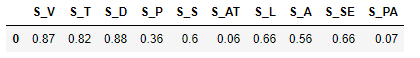
\includegraphics[scale=1.0]{Figures/student_context.PNG}
    \caption{Student context template}
    \label{chap5:sc_template}
\end{figure}

% \subsubsection{Content \label{chap5:content}}

\begin{table}[H]
    \centering
 \begin{tabular}{|p{3.8cm}|p{10.3cm}|} 
    \hline
    \textrm{\textbf{Content Context}} & \textrm{\textbf{Description}} \\ \hline
    \textrm{Ease of understanding (C\_E)} & \textrm{How relatively easy is it to understand the content?}\\ \hline
    \textrm{Simple/Intuition (C\_I)} & \textrm{Does it provide a surface level or deep understanding of the topic?} \\ \hline
    \textrm{Surface/In-depth (C\_ID)} & \textrm{How much preference is given to live experiments to help understand a concept?} \\ \hline
    \textrm{Brief/Concise (C\_C)} & \textrm{Is it short, to the point or descriptive, verbose and elaborative, keeping in mind that learners have different levels of concentration and capacity to remember?} \\ \hline
    \textrm{Thorough (C\_T)} & \textrm{How well does the content item cover the topic?} \\ \hline
    \textrm{Preference/Well reviewed/Well rated(C\_R)} & \textrm{How well rated is the explanation? } \\ \hline
    \textrm{Theoretical/Abstract (C\_A)} & \textrm{How theoretical or abstract is the content item?} \\ \hline
    \textrm{Practical/Hands on (C\_P)} & \textrm{Is it something that can be tried or experienced?} \\ \hline
    \textrm{Experimental/Task-based (C\_ETB)} & \textrm{Does it require a task to be completed to fully understand it, like collaboration with other students or some research/findings?} \\ \hline
    \end{tabular}
    \caption{Content context}
    \label{chap5:content}
\end{table}

% \subsubsection{An Example Data Point \label{chap5:datapoint}}

Below (Figure \ref{chap5:cc_template}) is a content context data point prepared for the course. This content item is thorough(\textit{C\_T}), practical(\textit{C\_P}), and experimentally sound(\textit{C\_ETB}), but not in-depth(\textit{C\_ID}),concise(\textit{C\_C}), and abstract(\textit{C\_A}). It is moderate in terms of  understanding(\textit{C\_E}), intuitiveness(\textit{C\_I}) and has positive reviews(\textit{C\_R}). \par

\begin{figure}[H]
    \centering
    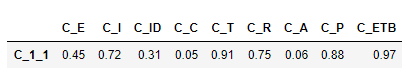
\includegraphics[scale=1.0]{Figures/content_context.PNG}
    \caption{Content context template}
    \label{chap5:cc_template}
\end{figure}

Apart from the above contextual data, there is a course which is taught. For our experiments, we consider a typical course which comprises of topics to be taught. These topics are labeled as \textit{ T\_1, T\_2 ... T\_25}. For e.g: T\_1 refers to the first topic of the course. Each topic has between 5 to 20 different content items. Each content is labeled in the format \textit{C}\_\textit{topic-id}\_\textit{content-number}. For e.g: C\_1\_2 refers to the second content item for topic T\_1. \par

We now have the required contextual information. Topics in the course are taught in a sequence outlined by the teacher. This allows them to control the course sequence. Let us take an example to understand the data.\par

\section{Environment \label{chap5:environment}}

We run a simulation of a course being taken by students with the omniscient policy and the learning algorithm deciding the content item to be presented for each student. It is an environment where several students are taking the course at the same time. Both the omniscient policy and the learning algorithm work in online mode. The learning algorithm updates it's parameters in each round to give better predictions. \par

\section{Evaluation Strategy \label{chap5:evaluationStrategy}}

Since there are no readily available benchmarks to compare our algorithm, we assume there exist an omniscient policy. This policy has optimal parameters to recommend the best arm to pull.  \par

We run the same course with an omniscient policy and the learning algorithm to evaluate our learning algorithm relative to the omniscient policy. The evaluation is conducted with and without skipping. Due to the stochastic nature of a student's feedback both the omniscient policy and the learning algorithm will run for a different number of rounds. However, the total cumulative reward available is the same for both of them. Hence we evaluate them based on cumulative reward accumulated over all rounds. \par 

We simulate the student feedback as a Bernoulli distribution. Here, the probability of success is the maximum expected reward computed by the omniscient policy. This reward for an arm $a$ with optimal parameters $\theta^{*}_{t,a}$ and with context vector $x_{t,a}$ at round $t$ is given by $E[r_{t,a}|\mathbf{x_{t,a}}] = x^{T}_{t,a}\mathbf{\theta^{*}_{t,a}}$. It is passed to the Bernoulli distribution as the probability of reward for the presented content item. Based on the reward received by the learning algorithm the arm parameters are updated to make better decisions in the upcoming rounds. This experiment aims to find how well does our algorithm optimize an arm's parameters to match the omniscient policy. \par

\section{Omniscient Policy \label{chap5:omniscientPolicy}}

This policy knows all the probability distributions. At every step of makes the way the best decision as it knows the true distributions. It does not have to learn anything. It has optimal parameters $\theta^*$ for each arm. Hence it is expected to maximize the cumulative reward.

This policy calculates the expected payoff for each arm $a$ available for a topic. It then selects the arm which has maximum expected payoff. 

\section{Learning Algorithm \label{chap5:learningAlgorithm}}

The learning algorithm can adapt to several students at the same time to present a content item personalized for each student. For every topic, a student is trying to learn it gets the expected payoff for all available content items. It checks whether it should skip to next topic or remain on the current topic. Skipping is activated only if the student gave no reward for a content item presented for the topic. \par

When a student is on a topic, the algorithm presents a content item that could maximize rewards. After working through the content item, the student shares feedback on the content item. If a reward is sent, then this implies that the student understood the concept and can be taken to the next topic. If no reward was sent, then the student may be presented with the next best content item for the same topic or could be moved to the next topic in the course sequence.\par 

Once the student has shared feedback on the content item, the data is sent to train the skip classifier to make a better prediction in forthcoming rounds. \par

\section{Skip Topic \label{chap5:skipTopics}}

The learning algorithm checks with skip topic feature to decide whether or not the content item should be presented for the current topic. Skip topic predicts this by using a student's context along with the estimated payoff for the current topic and the estimated payoff for the next topic in the course sequence. \par

It makes this decision using an online supervised learning stochastic gradient descent classifier with student context along with the estimated payoff of the current and next topic to make a decision. The label for the classifier depends on the reward received for the topic. If a reward was sent then the label is set to 0 or else it is set to 1. Thus the classifier makes use of the feedback sent by all students to recognize common topics and content items that students find difficult so it could make a confident decision. \par

The aim to create skip topic feature is to streamline learning for a student. If a student has been taught a topic once and was not satisfied with it, then there is the option to skip to the next topic or explain the same topic with a different content item. \par

The skip classifier is a linear support vector machine estimator with hinge loss. The estimator is a regularized linear model with stochastic gradient descent (SGD) learning. The gradient of the loss is estimated, each sample at a time and the model is updated along the way with a decreasing learning rate. The regularizer is a penalty added to the loss function that shrinks model parameters towards the zero vector using squared Euclidean norm \cite{scikit-learn}. \par
	\startchapter{Results and Evaluation}
\label{chapter:eval}

This chapter presents results using the experimental set-up given in the previous chapter (Chapter \ref{chapter:Exp}). We evaluate the learning algorithm with respect to the omniscient policy. Before evaluation we need to first find optimal values for hyper-parameters $\alpha$ (Section \ref{chap6:alpha}) and confidence threshold $C$ (Section \ref{chap6:threshold}). We then proceed to use these optimal values to evaluate the learning algorithm with and without the skip feature. (Section \ref{chap6:la}). 

% Up until now, we did not penalize content items which gave no rewards. However, in section \ref{chap6:pr} we penalize such content items.

\section{Confidence Bound $\alpha$ \label{chap6:alpha}}

Finding an optimal value for $\alpha$ is important to learn faster as it scales the confidence bound of each content item. An optimal value would find the right balance between exploration and exploitation. A higher value of $\alpha$ would imply the learning algorithm takes more rounds exploring which can lead to sub-optimal results. \par

This parameter is configured for the learning algorithm and not the omniscient policy. We empirically evaluated an optimal value for $\alpha$ using course 1 (Section: \ref{chap5:courses}). The graph (Figure \ref{chap6:rpr_alpha}) shows the cumulative reward for different values of $\alpha$. \par

% \begin{figure}[H]
%     \centering
%     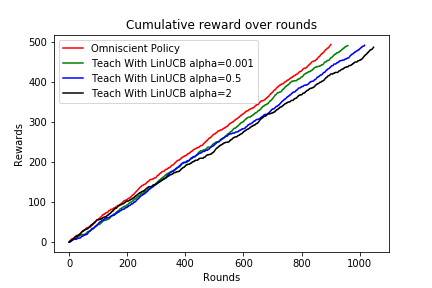
\includegraphics[scale=1.0]{Figures/optimal_alpha.png}
%     \caption{Cumulative reward per $\alpha$.}
%     \label{alpha}
% \end{figure}

\begin{figure}[H]
    \centering
    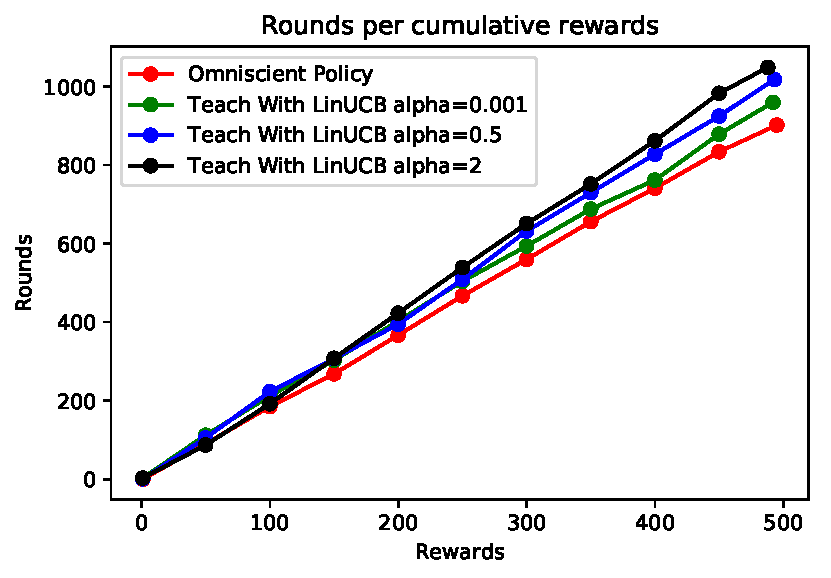
\includegraphics[scale=1.0]{Figures/rounds_per_reward_for_alpha.pdf}
    \caption{Rounds per cumulative reward for $\alpha$.}
    \label{chap6:rpr_alpha}
\end{figure}

The graph (Figure \ref{chap6:rpr_alpha}) compares the omniscient policy with the learning algorithm for different values of $\alpha$. It shows that the learning algorithm \textbf{took 960 rounds to maximize reward when} $\mathbf{\alpha = 0.001}$ compared to 1018 rounds required by $\alpha = 0.5$ and 1049 rounds required by $\alpha = 2$. On repeated run of the same experiment, we found that a value of $\alpha$ between 0 to 0.5 gives better results.\textbf{We would be using $\alpha = 0.001$ to evaluate the learning algorithm.} \par

The graph (Figure \ref{chap6:rprr_alpha}) presents a different view of the above graph. It shows the number of rounds to reward ratio at different intervals for different values of $\alpha$ and compares it to the omniscient policy. It clearly shows that $\alpha = 0.001$ required the fewest rounds to maximize reward. 

\begin{figure}[H]
	\centering
    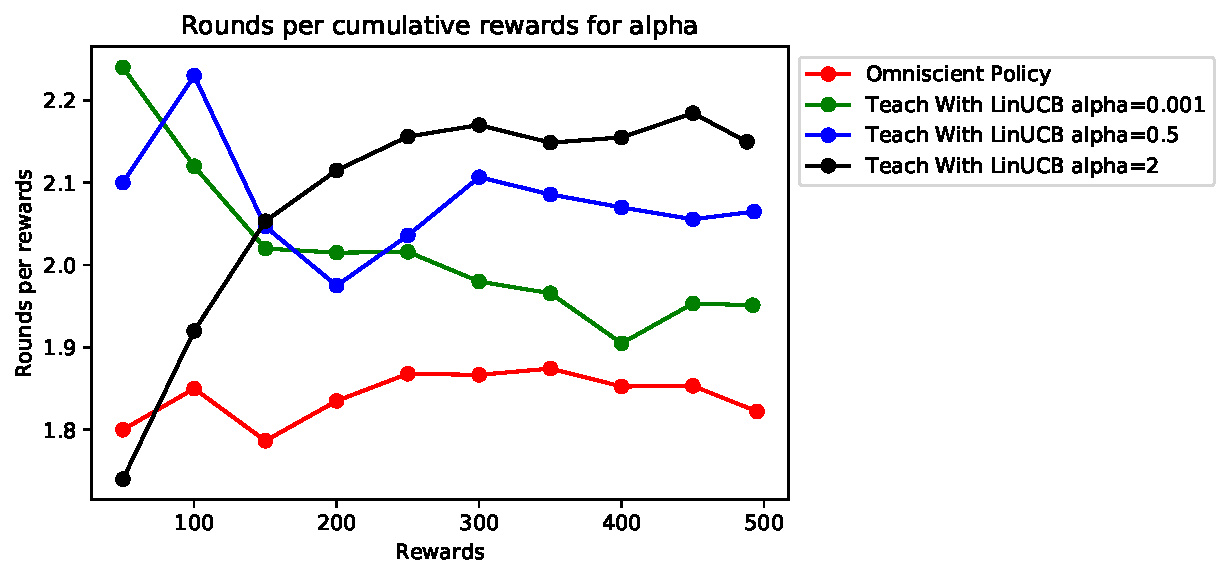
\includegraphics[scale=0.85]{Figures/rounds_per_reward_ratio_for_alpha.pdf}
    \caption{Rounds per cumulative reward ratio for $\alpha$.}
    \label{chap6:rprr_alpha}
\end{figure}

% The graph \ref{chap6:rpr_omni} presents a different view of the above graph. It shows the number of extra rounds required for different value's of $\alpha$ compared to the omniscient policy. It clearly shows that $\alpha = 0.001$ required the fewest rounds to maximize reward. 

% \begin{figure}[H]
%     \centering
%     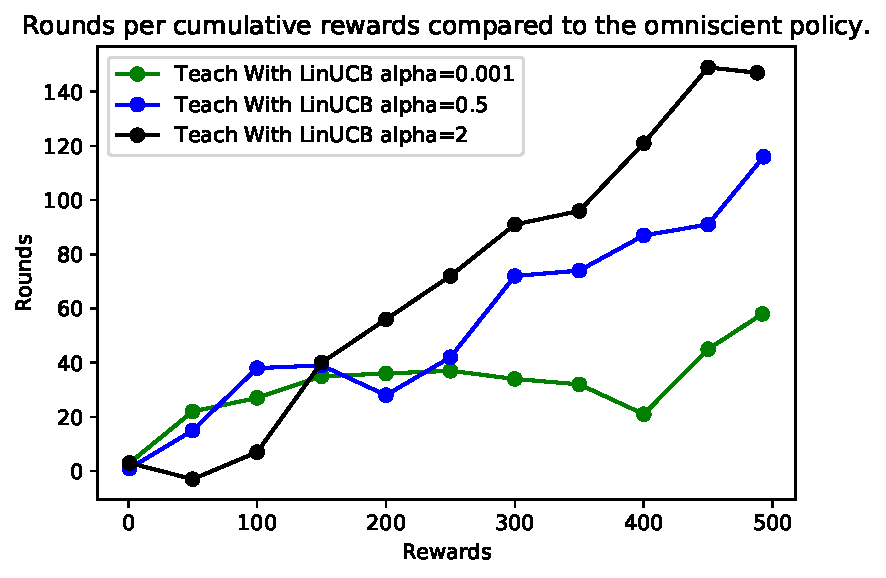
\includegraphics[scale=1.0]{Figures/rounds_per_rewards_wrt_omni.pdf}
%     \caption{Rounds per cumulative reward compared to the omniscient policy.}
%     \label{chap6:rpr_omni}
% \end{figure}

The below table shows the number of content items presented for different values of $\alpha$. As $\alpha$ increases more content items are presented for a student to learn.

\begin{table}[h]
    \centering
 \begin{tabular}{|c|c|}
    \hline
    \textrm{\textbf{Values of $\alpha$}} & \textrm{\textbf{Content Items Explored}} \\ \hline
     \textrm{0.001} & \textrm{64}\\ \hline
     \textrm{0.5} & \textrm{79}\\ \hline
     \textrm{2.0} & \textrm{81}\\ \hline
    \end{tabular}
    \caption{Content items explored per $\alpha$}   \label{chap6:content_items_for_alpha_without_penalty}
\end{table}. 

\section{Confidence Threshold (C)
\label{chap6:threshold}}

This is a threshold on the confidence score the skip classifier should exceed for its prediction to be accepted. Skipping is enabled for a topic only after a student gives no reward to a content item. The threshold helps: 
\begin{itemize}
\item To keep a student engaged by skipping topics they are unable to understand.
\item Give teachers control on their preference to skipping. 
\item Allow the learning algorithm to skip content items that are less likely to give rewards.
\end{itemize}
 
We do not want the confidence threshold to be too high as students might have to go through each content item nor do we want it to be too low such that students are taken to the next topic on the first occurrence of not understanding a topic. Hence finding an optimal value for the confidence threshold is important to have a good learning experience. 

We evaluate the performance for different values of the confidence threshold over course 1 (Section: \ref{chap5:courses}). Below are the results. 

\subsection{Without confidence threshold} 

We evaluated the skip classifier with no confidence threshold. Below is a table that shows the results. 

\begin{table}[h]
    \centering
    \begin{tabular}{l|l|c|c|c}
    \multicolumn{2}{c}{}&\multicolumn{2}{c}{Reward per prediction type (in \%).}&\\
    \cline{3-4}
    \multicolumn{2}{c|}{}&Stay (0) &Skip (1)&\multicolumn{1}{c}{Total}\\
    \cline{2-4}
    \multirow{2}{*}{Reward}& 0 & $25.10$ & $18.28$ & $43.38$\\
    \cline{2-4}
    & 1 & $32.25$ & $24.37$ & $56.62$\\
    \cline{2-4}
%     \multicolumn{1}{c}{} & \multicolumn{1}{c}{Total} & \multicolumn{1}{c}{$160$} & \multicolumn{1}{c}{$119$} & \multicolumn{1}{c}{$558$}\\
    \end{tabular}
    \caption{Predictions without confidence threshold}
\end{table}

The classifier is evaluated on how well it helps the learning algorithm maximize reward. This shows us that by \textbf{56.62\%} it's decision helped increase reward. \par 

\subsection{With confidence threshold}

We evaluate the skip classifier with confidence threshold. We will only consider data points where the classifier's decision was overruled as its confidence score was below the threshold. This would be when the classifier had predicted skipping to the next topic, but since the confidence score was below the threshold, the prediction was ignored. This gives us the true measure of effectiveness for the confidence threshold.\par  

We evaluated the classifier for different values of confidence threshold. For different threshold values performance ranged consistently between 56 - 60 \%. We found the skip classifier performed most optimally when the confidence threshold is 30. The below table \ref{CT_opt} shows the results. 

\begin{table}[H]
    \centering
\begin{tabular}{l|l|c|c|c}
\multicolumn{2}{c}{}&\multicolumn{2}{c}{Reward per prediction type (in \%).}&\\
\cline{3-4}
\multicolumn{2}{c|}{}&Stay (0) &Skip (1)&\multicolumn{1}{c}{Total}\\
\cline{2-4}
\multirow{2}{*}{Reward}& 0 & $18.3$ & $24.18$ & $42.48$\\
\cline{2-4}
& 1 & $18.3$ & $39.22$ & $57.52$\\
\cline{2-4}
% \multicolumn{1}{c}{} & \multicolumn{1}{c}{Total} & \multicolumn{1}{c}{$56$} & \multicolumn{1}{c}{$97$} & \multicolumn{1}{c}{$316$}\\
\end{tabular}
\caption{Predictions with confidence threshold of 10}
\label{CT_opt}
\end{table}

The above table shows us that by \textbf{57.52\%} its decision helped increase reward. As the value of the confidence threshold was increased the number of skips decreased. Table \ref{threshold_30} shows the results for confidence threshold of 30.

\begin{table}[H]
    \centering
    \begin{tabular}{l|l|c|c|c}
    \multicolumn{2}{c}{}&\multicolumn{2}{c}{Reward per prediction type (in \%).}&\\
    \cline{3-4}
    \multicolumn{2}{c|}{}&Stay (0) &Skip (1)&\multicolumn{1}{c}{Total}\\
    \cline{2-4}
    \multirow{2}{*}{Reward}& 0 & $36.82$ & $4.09$ & $40.91$\\
    \cline{2-4}
    & 1 & $50.45$ & $8.64$ & $59.09$\\
    \cline{2-4}
%     \multicolumn{1}{c}{} & \multicolumn{1}{c}{Total} & \multicolumn{1}{c}{$192$} & \multicolumn{1}{c}{$28$} & \multicolumn{1}{c}{$440$}\\
    \end{tabular}
\caption{Predictions with confidence threshold of 30}
\label{threshold_30}
\end{table}

The above table shows us that by \textbf{59.09\%} it's decision helped increase reward.\par

\section{Learning Algorithm \label{chap6:la}}

We now evaluate the learning algorithm with and without the skip feature. 

\subsection{Without Skipping}

With skipping disabled the only way a student can move to the next topic is by understanding it or until all content items have failed to explain the student. This could increase the number of rounds required by a student to complete a course. \par 

The graph (Figure \ref{cr_withoutSkip}) shows the cumulative reward of the learning algorithm with respect to the omniscient policy. The reward for the omniscient policy increases linearly, whereas that of the learning algorithm is similar to the optimal policy. This is expected as it does not have optimal arm parameters pre-configured and learns them in each round. 

% \begin{figure}[h]
%     \centering
%     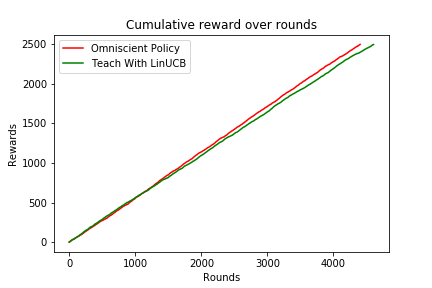
\includegraphics[scale=1.0]{Figures/cum_reward_optimal_without_confidence_threshold.png}
%     \caption{Cumulative reward without skipping.}
%     \label{cr_withoutSkip}
% \end{figure}

\begin{figure}[h]
    \centering
    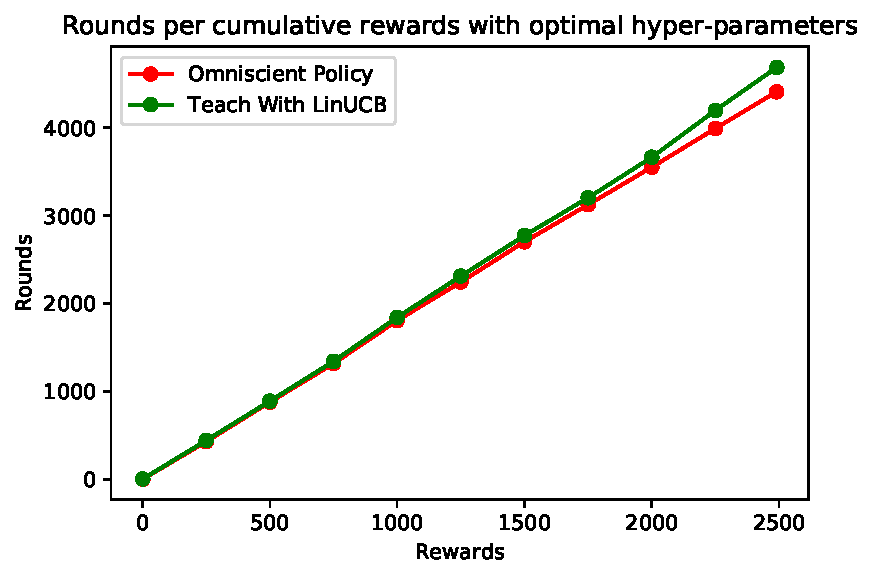
\includegraphics[scale=1.0]{Figures/rounds_per_reward_no_skipping.pdf}
    \caption{Rounds per cumulative reward without skipping.}
    \label{cr_withoutSkip}
\end{figure}

The omniscient policy required 4410 rounds to get a cumulative reward of 2490. This implies it needs 1.77 rounds for a reward (of 1). The learning algorithm required 4688 rounds to get a reward of 2491. This implies it needs 1.88 rounds for a reward (of 1). The graph (Figure \ref{chap6:rprr_no_skip}) shows the number of rounds per reward required by the algorithm at different intervals with optimal values of hyper-parameters and compares it to the omniscient policy. It shows that our learning algorithm is close to the optimal policy. \par

\begin{figure}[H]
    \centering
    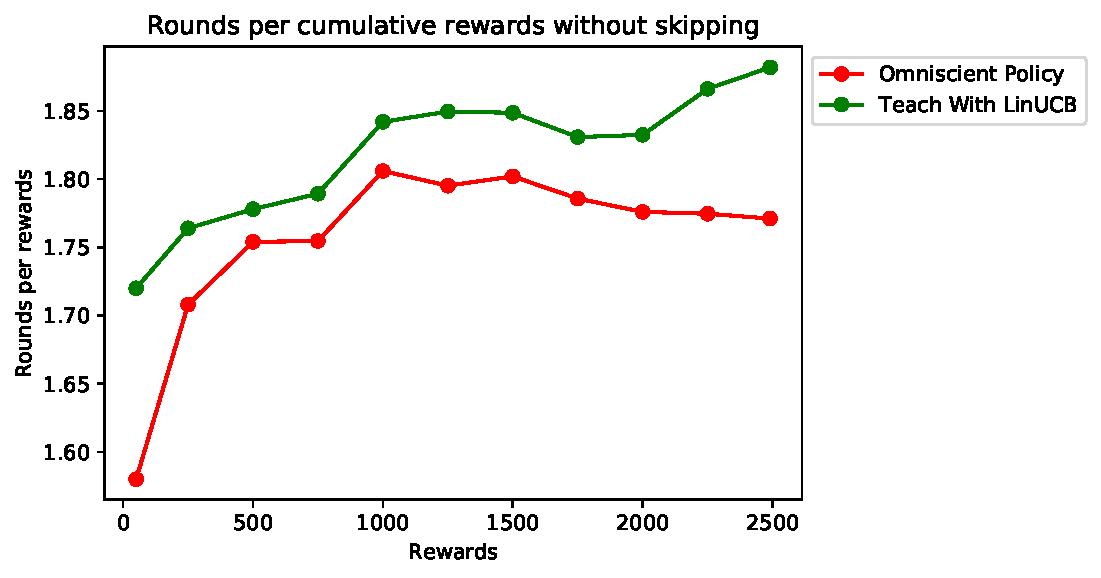
\includegraphics[scale=0.95]{Figures/rounds_per_reward_ratio_no_skipping.pdf}
    \caption{Rounds per cumulative reward ratio without skipping.}
    \label{chap6:rprr_no_skip}
\end{figure}

\subsection{With Skipping}

If a topic is not understood by a student then skipping is enabled. This does not directly imply the student would be taken to the next topic. For it to happen, the skip classifier should be confident beyond the confidence threshold to predict that it would be better to take the student to the next topic. \par 

Skipping tells the learning algorithm to skip sub-optimal content items and instead move to content items that have a higher estimated reward. This ensures that we do not present content items which are unlikely to help a student understand the topic. The graph (Figure \ref{cr_withSkip}) shows results of the learning algorithm with optimal confidence threshold $C = 30$ and $\alpha = 0.001$.

\begin{figure}[H]
    \centering
    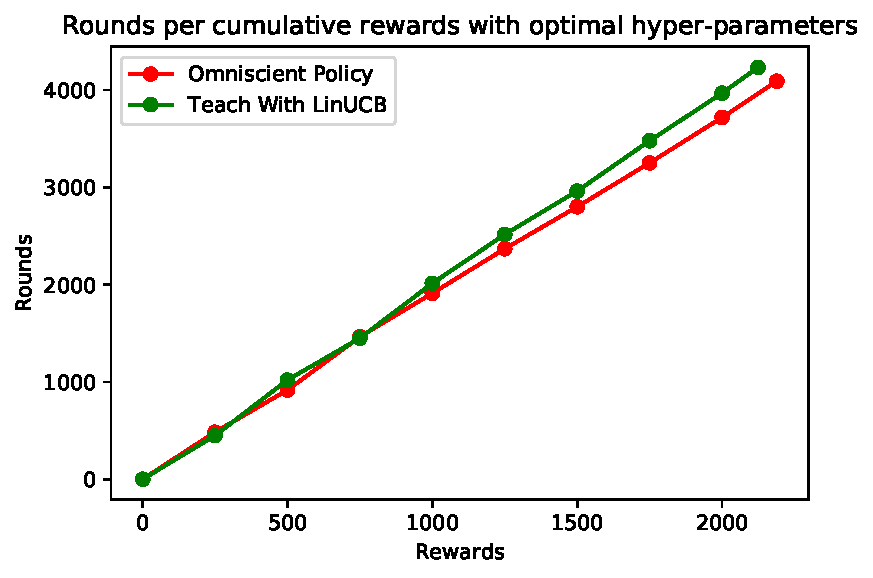
\includegraphics[scale=1.0]{Figures/rounds_per_reward_with_skipping.pdf}
    \caption{Rounds per cumulative reward with skipping}
    \label{cr_withSkip}
\end{figure}

% \begin{figure}[H]
%     \centering
%     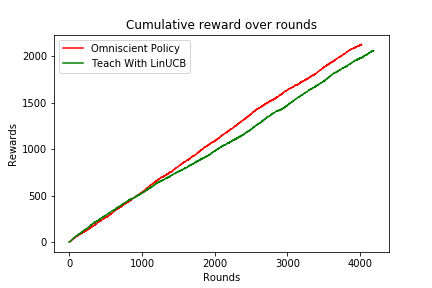
\includegraphics[scale=1.0]{Figures/cum_reward_small.png}
%     \caption{Cumulative reward with skipping}
%     \label{cr_withSkip}
% \end{figure}

The graph (Figure \ref{cr_withSkip}) shows the performance of the learning algorithm with respect to the omniscient policy. The number of rounds and the cumulative reward reduces with skipping enabled. The cumulative reward reduces as for topics that a student did not understand the skip classifier predicted with high confidence that it would be better to move to the next topic. \par

The omniscient policy required 4019 rounds to get a cumulative reward of 2128. This implies it needs 1.89 rounds for a reward (of 1). The learning algorithm required 4185 rounds to get a reward of 2062. This implies it needs 2.03 rounds for a reward (of 1). The graph (Figure \ref{chap6:rprr_skip}) shows the number of rounds per reward required by the algorithm at different intervals for optimal values of hyper-parameters and compares it to the omniscient policy. It shows that even with skipping our learning algorithm is close to the optimal policy. \par

\begin{figure}[H]
    \centering
    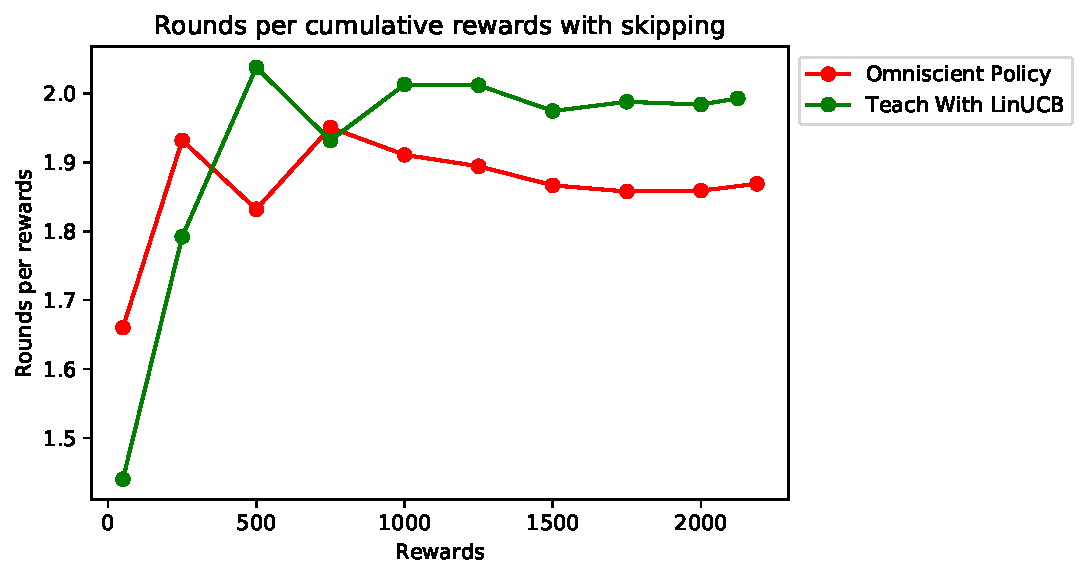
\includegraphics[scale=0.95]{Figures/rounds_per_reward_ratio_with_skipping.pdf}
    \caption{Rounds per cumulative reward ratio with skipping.}
    \label{chap6:rprr_skip}
\end{figure}

Comparing the cumulative reward graph with and without skipping shows us that our learning algorithm performs better without skipping than with skipping. However, without skipping it needs more rounds which could affect student experience. \par

% \section{Penalizing Rewards \label{chap6:pr}}

% We now update our reward assignment strategy to penalize content items which gave no rewards. This presents a different perspective as earlier in Section \ref{chap6:la} we did not penalize content items which gave no rewards. In this section rewards received by content items change from $\{0,1\}$ to $\{-1,1\}$. \par

% When content items receive no reward, the learning algorithm reduces the estimated expected reward from it. This reduces the possibility of such content items being selected which results in more content items being explored as seen in table \ref{chap6:content_items_for_alpha_with_penalty}. \par

% We follow a similar approach as before. We first find the optimal values for the hyper-parameters before we evaluate our learning algorithm. \par

% \subsection{Comparing $\alpha$}

% $\alpha$ is a scaling factor to control exploration. A higher value of $\alpha$ reduces cumulative reward as more rounds are spent exploring to find the optimal content items. The graph below shows the cumulative reward for different values of $\alpha$. 

% \begin{figure}[H]
%     \centering
%     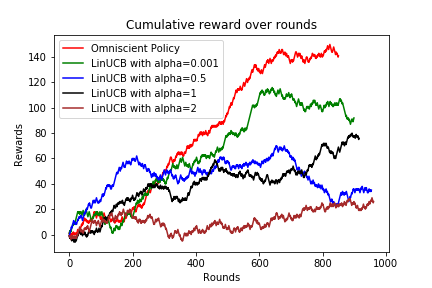
\includegraphics[scale=1.0]{Figures/penalty/cum_reward_compare_alphas.png}
%     \caption{Cumulative penalized rewards per alpha}
%     \label{cr_withSkip}
% \end{figure}

% As before $\alpha=0.001$ gives the best results compared to the omniscient policy. Below is the table which shows the number of content items explored for different values of $\alpha$. 

% \begin{table}[h]
%     \centering
%  \begin{tabular}{|c|c|}
%     \hline
%     \textrm{\textbf{Values of $\alpha$}} & \textrm{\textbf{Content Items Explored}} \\ \hline
%      \textrm{0.001} & \textrm{75}\\ \hline
%      \textrm{0.5} & \textrm{89}\\ \hline
%      \textrm{1.0} & \textrm{104}\\ \hline
%      \textrm{2.0} & \textrm{105}\\ \hline
%     \end{tabular}
%     \caption{Content items explored per $\alpha$}
%   \label{chap6:content_items_for_alpha_with_penalty}
% \end{table}

% \subsection{Confidence Threshold}

% We ran a simulation over Course 1 to find the optimal value of confidence threshold $C$. An optimal value would be one for which the skip classifier has the best performance. We ran experiments for different values of confidence threshold. The table \ref{chap6:confusion_matrix_without_ct} shows the results of the predictions made by the skip classifier with no threshold set.\par


% \begin{table}[h]
%     \centering
%     \begin{tabular}{l|l|c|c|c}
%     \multicolumn{2}{c}{}&\multicolumn{2}{c}{Predictions}&\\
%     \cline{3-4}
%     \multicolumn{2}{c|}{}&Stay (0) &Skip (1)&\multicolumn{1}{c}{Total}\\
%     \cline{2-4}
%     \multirow{2}{*}{Reward}& 0 & $74$ & $39$ & $113$\\
%     \cline{2-4}
%     & 1 & $82$ & $64$ & $146$\\
%     \cline{2-4}
%     \multicolumn{1}{c}{} & \multicolumn{1}{c}{Total} & \multicolumn{1}{c}{$156$} & \multicolumn{1}{c}{$103$} & \multicolumn{1}{c}{$518$}\\
%     \end{tabular}
%     \caption{Confusion matrix without confidence threshold}
%     \label{chap6:confusion_matrix_without_ct}
% \end{table}

% Without any threshold, our classifier would have an accuracy of 56.37 \%. The table \ref{chap6:confusion_matrix_with_ct20} shows the results for the classifier for confidence threshold of 20. This gives better results. 

% \begin{table}[h]
%     \centering
%     \begin{tabular}{l|l|c|c|c}
%     \multicolumn{2}{c}{}&\multicolumn{2}{c}{Predictions}&\\
%     \cline{3-4}
%     \multicolumn{2}{c|}{}&Stay (0) &Skip (1)&\multicolumn{1}{c}{Total}\\
%     \cline{2-4}
%     \multirow{2}{*}{Reward}& 0 & $41$ & $20$ & $61$\\
%     \cline{2-4}
%     & 1 & $59$ & $39$ & $98$\\
%     \cline{2-4}
%     \multicolumn{1}{c}{} & \multicolumn{1}{c}{Total} & \multicolumn{1}{c}{$100$} & \multicolumn{1}{c}{$59$} & \multicolumn{1}{c}{$257$}\\
%     \end{tabular}
%     \caption{Confusion matrix with confidence threshold of 20}
%     \label{chap6:confusion_matrix_with_ct20}
% \end{table}

% With a threshold set to it, our classifier would have an accuracy of 61.64\%.

% \subsection{Learning Algorithm}

% We now configure these optimal values and run a simulation of Course 2 for both the omniscient policy and the learning algorithm.  The omniscient policy knows the best arm to pull in each round. On the other hand, our learning algorithm explores to find the best content item.

% \subsubsection{No Skipping}

% We now evaluate our learning algorithm without skipping. 

% \begin{figure}[H]
%     \centering
%     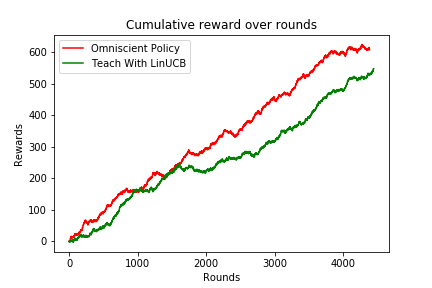
\includegraphics[scale=1.0]{Figures/penalty/cum_reward_small_NO_SKIPPING.png}
%     \caption{Cumulative penalized rewards without skipping}
%     \label{cr_withoutSkip}
% \end{figure}

% The omniscient policy took 4384 rounds compared to 4443 taken by the learning algorithm to complete the course for all students. The rewards accumulated by the omniscient policy is 608 compared to 547 by the learning algorithm. The learning algorithm performs sub-optimally, which is expected. 

% \subsubsection{With Skipping}

% With skipping enabled the ability of the learning algorithm to optimize its content item selection strategy is restricted. Skipping restricts the learning algorithm from exploring different content items to find the optimal content item in each round. The graph below shows the performance of the learning algorithm with respect to the omniscient policy with skipping enabled.

% \begin{figure}[H]
%     \centering
%     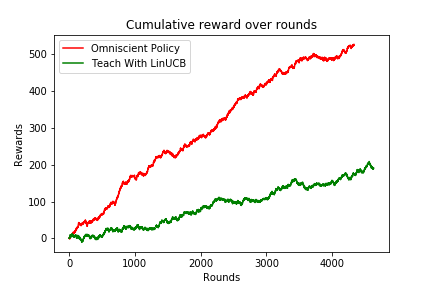
\includegraphics[scale=1.0]{Figures/penalty/cum_reward_small-WITH-SKIPPING.png}
%     \caption{Cumulative penalized rewards with skipping}
%     \label{cr_withSkip}
% \end{figure}

% The omniscient policy took 4335 rounds compared to 4634 taken by the learning algorithm to complete the course for all students. The rewards accumulated by the omniscient policy is 527 compared to 191 received by the learning algorithm. The learning algorithm performs poorly, when exploration is restricted. \par 

% With this experiment, we find that skipping although useful should only be introduced once the learning algorithm has sufficiently explored all content items. If introduced too early then skipping prevents the learning algorithm from exploring. However if introduced too late then its value diminishes. 
 
% Future Work 

% We need to come up with an approach to introduce skipping once the learning algorithm has explored sufficiently. 


% Additional optimizations 

% - Decaying confidence threshold. 
% - Pre-trained skip classifier leads to better performance. 
% - Analysis over datasets of different sizes. 
	\startchapter{Conclusions}
\label{concl}

This project presents a student-centric approach to teaching. An approach which could make a classroom more interactive by providing a personalized learning experience for students. We synthesized an unbiased dataset to represent heterogeneous student and content data to evaluate our learning algorithm. Since there is no benchmark available, we created an omniscient policy which has optimal parameters pre-configured. The algorithm learns these parameters to find an optimal content item for each student. \par 

We then present a feature which would be useful when there are several different content items for a topic to avoid a student from getting frustrated by being unable to understand a topic. This not only helps students but also helps teachers recognize topics students are less likely to understand. We evaluated the learning algorithm to set a baseline for this new teaching methodology. \par 

Our future work would involve creating an actual course that follows the teaching methods outlined in this project. This would give real-world student data to evaluate the algorithm. We would also like to design other algorithms to evaluate their performance against our baseline algorithm. An additional optimization would be to find an optimal strategy to introduce skipping such that it does not restrict exploration and still provides a good student experience. \par
 	
%	\appendix
	%\startappendix{Additional Information}
\label{chapter:appendix}

1. Put Teacher's View up here.
2. LinUCB with references. 
3. 


This is a good place to put tables, lots of results, perhaps all the data compiled in the experiments. By avoiding putting all the results inside the chapters themselves, the whole thing may become much more readable and the various tables can be linked to appropriately.

The main purpose of an Appendix however should be to take care of the future readers and researchers. This implies listing all the housekeeping facts needed to continue the research. For example: where is the raw data stored? where is the software used? which version of which operating system or library or experimental equipment was used and where can it be accessed again?

Ask yourself: if you were given this thesis to read with the goal that you will be expanding the research presented here, what would you like to have as housekeeping information and what do you need? Be kind to the future graduate students and to your supervisor who will be the one stuck in the middle trying to find where all the stuff was left!



% The style of bibliography exemplified here is the "plain",
% normally used in science theses. This is shown
% by the entry {plain} below. Substitute the
% appropriate bibliography style. See also the
% PDF file "InformationOnBibliographyStyles" in this
% directory for more choices.

% The Bibliography file is a BibTex file named
% UVicThesis.bib and called below

	\TOCadd{Bibliography}
	\bibliographystyle{plain}
	\bibliography{UvicThesis}

\end{document}
